\documentclass{beamer}
\title{Hello, \textsc{beamer}!}
\author{Jaeho Lee}
\date{\today}
\begin{document}
\maketitle
\begin{frame}
  \frametitle{First Slide}
  \begin{itemize}
    \item TikZ
    \item Beamer
      \begin{itemize}
        \item Fun
        \item Cool
        \item Sexy
      \end{itemize}
  \end{itemize}
\end{frame}
\begin{frame}{Second Slide}
  \begin{enumerate}
    \item item1
    \item item2
  \end{enumerate}
  \begin{enumerate}[(a)]
    \item item1
    \item item2
  \end{enumerate}
  \begin{description}
    \item[key] value
    \item[long key] value
  \end{description}
\end{frame}
\begin{frame}{Third Slide}
  \begin{columns}
    \begin{column}{0.5\textwidth}
      \LARGE LEFT
    \end{column}
    \begin{column}{0.5\textwidth}
      \LARGE RIGHT
    \end{column}
  \end{columns}
  \vspace{2cm}
  \begin{center}
    \begin{tabular}{ccc}
      cell 1 & cell 2 & cell 3\\
      cell 4 & cell 5 & cell 6
    \end{tabular}
  \end{center}
\end{frame}
\begin{frame}{Fourth Slide}
  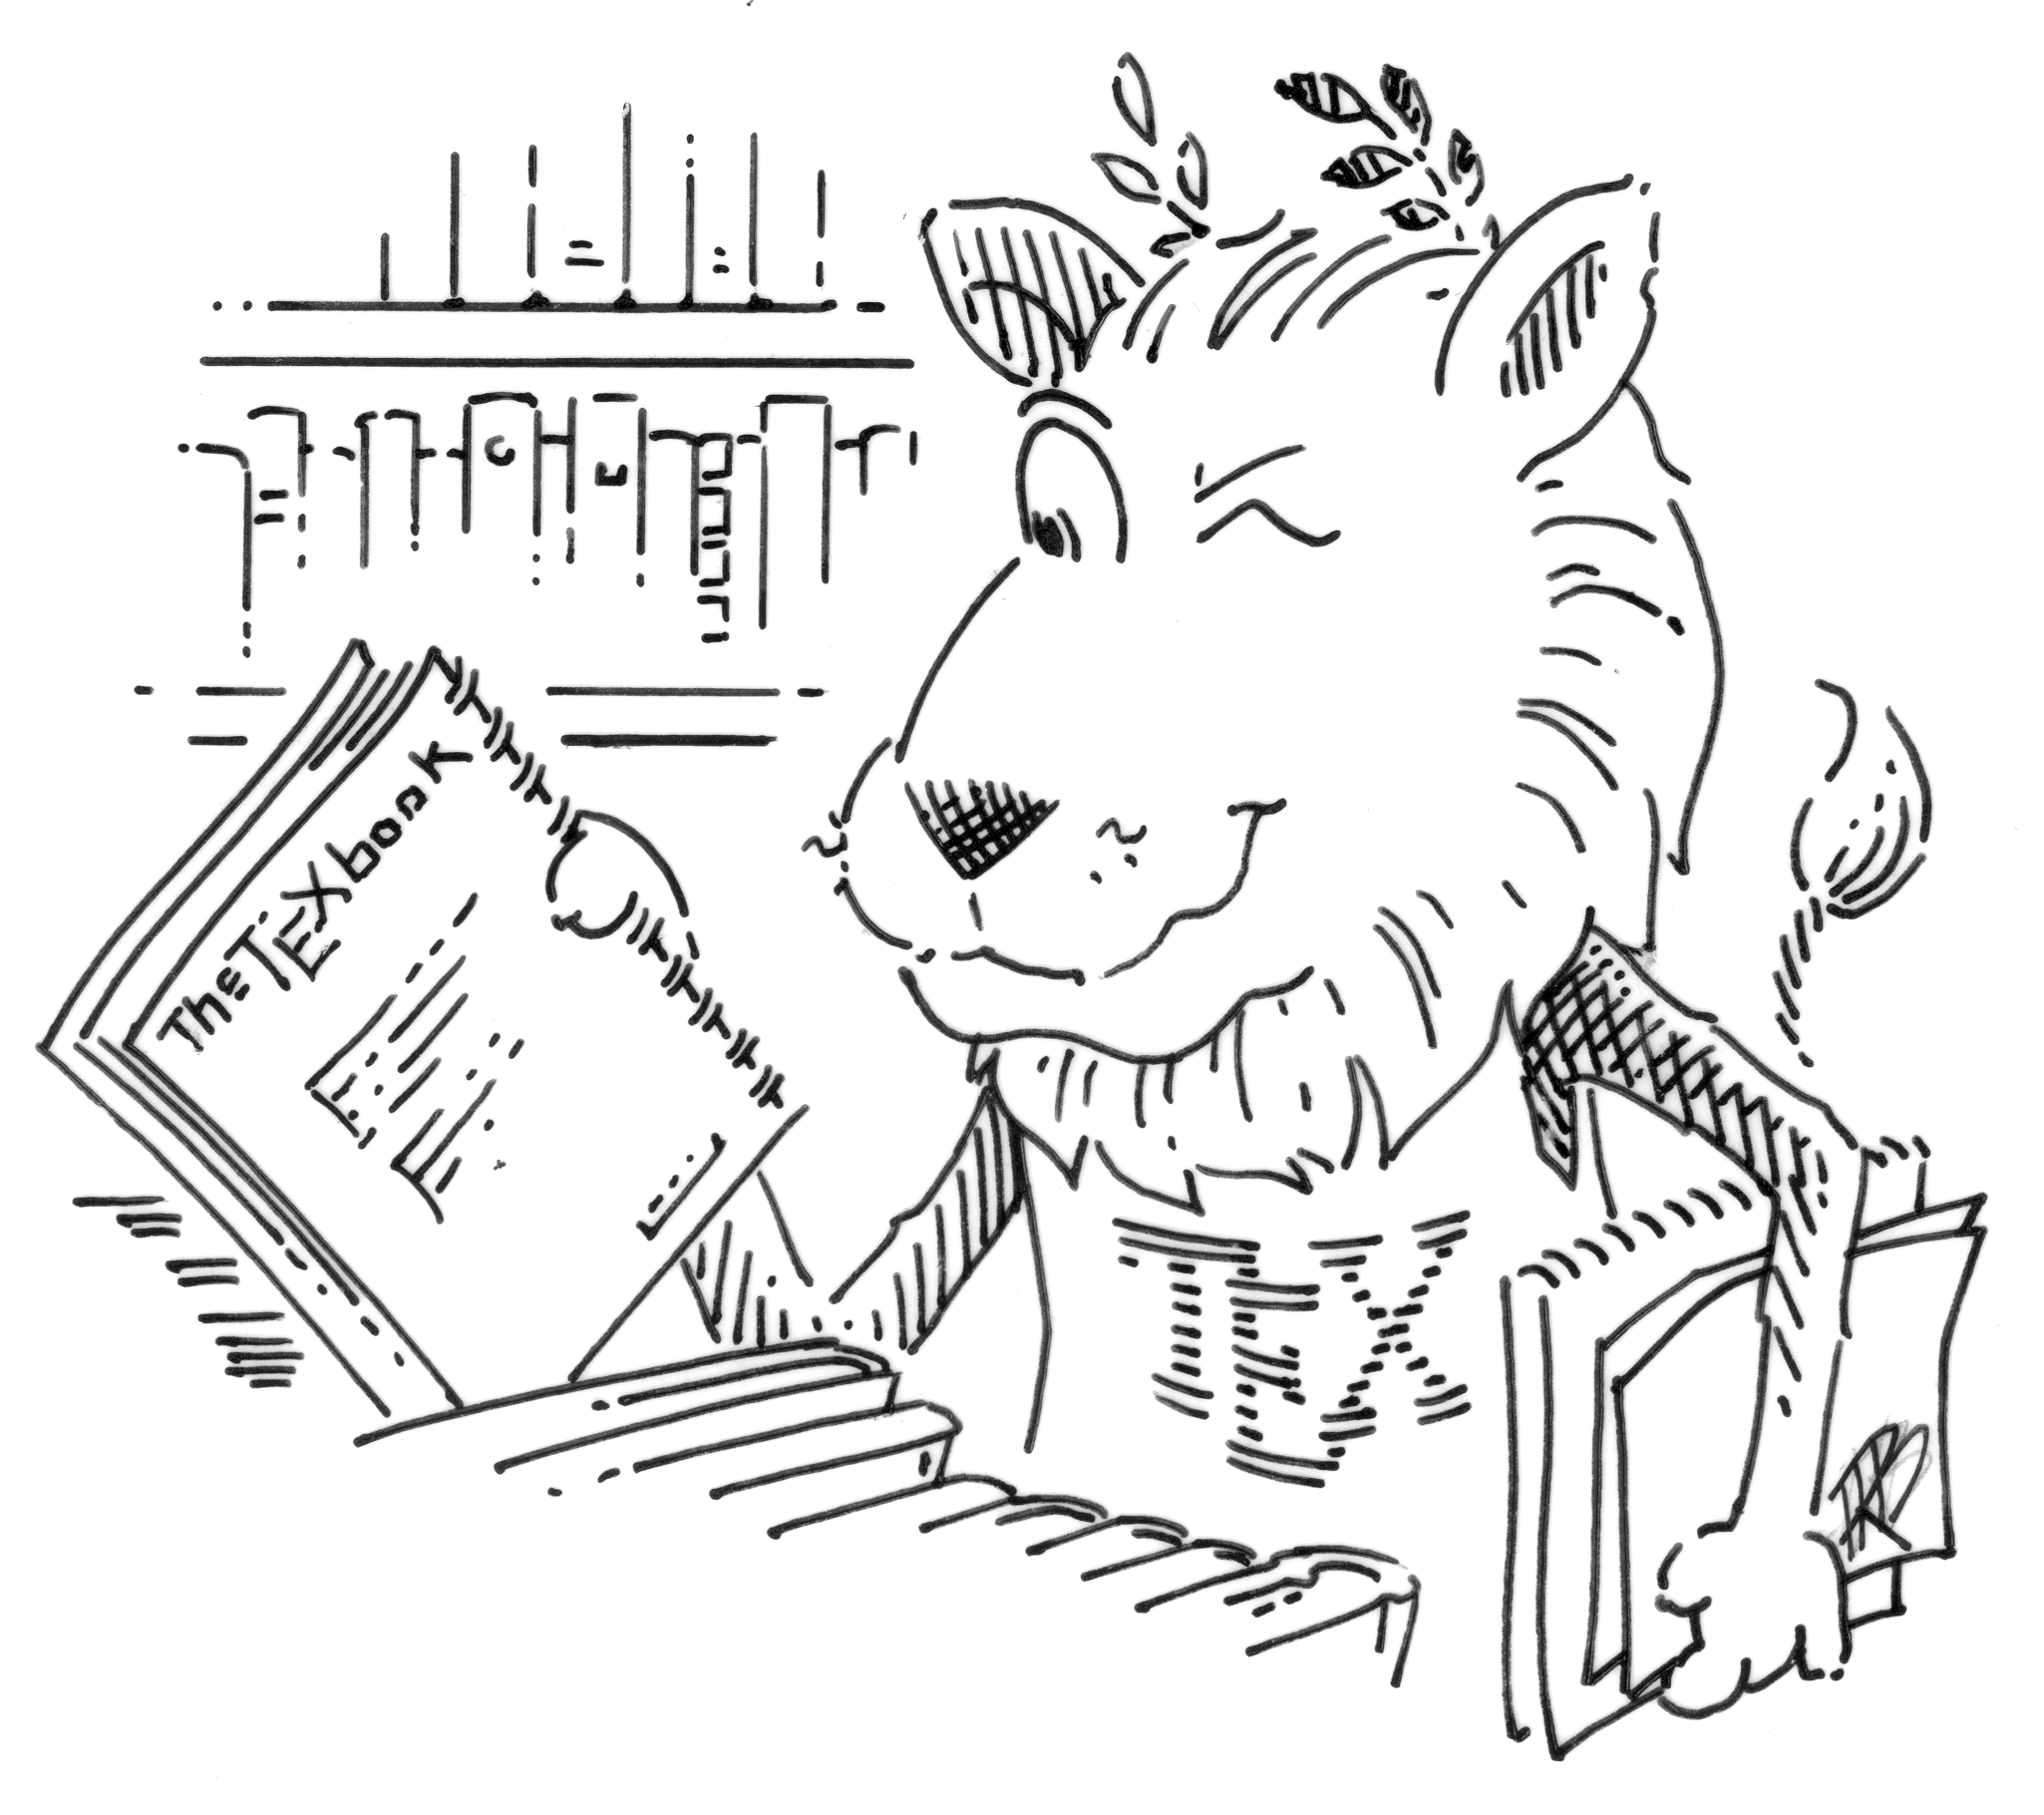
\includegraphics[width=\textwidth]{tex-lion}
\end{frame}
\begin{frame}{Fifth Slide}
  \begin{block}{Basis}
    If a subspace $W$ of a vector space $V$ is generated by a linearly
    independent $\mathcal B = \{\vec v_1, \dots, \vec v_k\} \subset V$, i.e.,
    \begin{equation*}
      \alert{W = \textrm{Span}\,\mathcal B},
    \end{equation*}
    $\mathcal B$ is called a \alert{basis} of $W$.
  \end{block}
  \begin{theorem}[Dimension Theorem]
    If $W$ is a \alert{finitely generated} subspace of a vector space $V$,
    any basis of $W$ has a \alert{same number of elements}.
    The number of elements of a basis of $W$ is called the \alert{dimension} 
    of $W$, and denoted \alert{$\dim W$}.
  \end{theorem}
\end{frame}
\end{document}
